\documentclass[a4paper,12pt,fleqn]{article}
\usepackage{fixltx2e}
\usepackage[utf8]{inputenc}
\usepackage{graphicx}
\usepackage{sidecap}
\usepackage{fancyhdr}
\usepackage{amssymb,mathtools}
\usepackage[swedish]{babel}
\usepackage[margin=1.5in]{geometry}
\usepackage{abstract}
\usepackage[parfill]{parskip}
\usepackage{tocloft}
\usepackage{adjustbox}
\usepackage{textcomp}
\usepackage[T1]{fontenc}
\usepackage{listings}
\usepackage{xcolor,colortbl}
\usepackage{hyperref}

%----------------------------------------------------------------
%C-kod formatering

\definecolor{listinggray}{gray}{0.9}
\definecolor{lbcolor}{rgb}{0.9,0.9,0.9}
\lstset{
backgroundcolor=\color{lbcolor},
    tabsize=4,    
%   rulecolor=,
    language=[GNU]C++,
        basicstyle=\scriptsize,
        upquote=true,
        aboveskip={1.5\baselineskip},
        columns=fixed,
        showstringspaces=false,
        extendedchars=false,
        breaklines=true,
        prebreak = \raisebox{0ex}[0ex][0ex]{\ensuremath{\hookleftarrow}},
        frame=single,
        numbers=left,
        showtabs=false,
        showspaces=false,
        showstringspaces=false,
        identifierstyle=\ttfamily,
        keywordstyle=\color[rgb]{0,0,1},
        commentstyle=\color[rgb]{0.026,0.112,0.095},
        stringstyle=\color[rgb]{0.627,0.126,0.941},
        numberstyle=\color[rgb]{0.205, 0.142, 0.73},
%        \lstdefinestyle{C++}{language=C++,style=numbers}’.
}
\lstset{
    backgroundcolor=\color{lbcolor},
    tabsize=4,
  language=C++,
  captionpos=b,
  tabsize=3,
  frame=lines,
  numbers=left,
  numberstyle=\tiny,
  numbersep=5pt,
  breaklines=true,
  showstringspaces=false,
  basicstyle=\footnotesize,
%  identifierstyle=\color{magenta},
  keywordstyle=\color[rgb]{0,0,1},
  commentstyle=\color{Darkgreen},
  stringstyle=\color{red}
  }
  %-----------------------------------------------------------------
  %marginaler

  \renewcommand{\abstractnamefont}{\normalfont\normalsize\bfseries}
  \renewcommand{\abstracttextfont}{\normalfont\small}
  \renewcommand{\headrulewidth}{0pt}
  \renewcommand{\cftsecleader}{\cftdotfill{\cftdotsep}} 
  \setlength{\absleftindent}{0pt}
  \setlength{\absrightindent}{0pt}
  \setlength{\headheight}{15pt}

  \addtolength{\oddsidemargin}{-.5in}
  	\addtolength{\evensidemargin}{-.5in}
  	\addtolength{\textwidth}{1in}


  %-----------------------------------------------------------------
  %header and footer

  \pagestyle{fancy}
  \lhead{
  	\begin{picture}(0,0)
  		\put(5,0){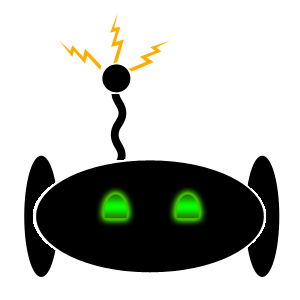
\includegraphics{logotyp.png}}
  	\end{picture}}
	
  \fancyhead[C]{\small{Mapmaster2001}}
  \fancyhead[R]{\small \today}
  \fancyfoot[L]{\small{TSEA56 \\ LIPS Kappa}}
  \fancyfoot[C]{\small{\thepage}}
  \fancyfoot[R]{\small{Projektgrupp 8 \\ mapmaster2001@cyd.liu.se}}

  %-----------------------------------------------------------------

%-------------------------------------------------------------------
%Första sidan

\begin{document}
	\pagestyle{fancy}
	 \pagenumbering{gobble}
	\vspace*{\fill}
		\begingroup
			\begin{center}
				\huge{\textbf{Simultan positionering och kartläggning}}
				\\
				\vspace{10pt}
				\normalsize
				Tobias Grundström och Hans-Filip Elo
				\\
				Kandidatprojekt Y - Grupp 8 - VT2014
				\\
				Version 0.4
				\end{center}
		\endgroup
	\vspace*{\fill}

	\begin{center} %Börjar centrering 
		Status
		\\
		\vspace{3pt} %Whitespace 3 pts
	    \begin{tabular}{| p{3cm} | p{3cm} | p{3cm} |} %tabell, 4 horizontella |, 3 cm emellan dem.
	    \hline %översta horizontella linjen.
	    Granskad & hanel742 & \today \\ \hline % & -tecken för att "gå till nästa ruta" 
		Godkänd & - & - \\ \hline % avslutas med \\ och \hline.

	    \end{tabular}
	\end{center}
	\vspace{2cm}
	\newpage
%-----------------------------------------------------------------
%Projektidentitet


	\vspace*{\fill}
		\begingroup
			\begin{center}
				\pagenumbering{roman}
				\LARGE{\textbf{PROJEKTIDENTITET}}
				\\
				\footnotesize
				Grupp 8, 2014/VT, MapMaster2001
				\\
				Linköpings tekniska högskola, Institutionen för Systemteknik (ISY)
				\\
				\vspace{1cm}
	  \begin{tabular}{| p{3cm} | p{4.3cm} | p{2.4cm} | p{3.8cm} |}
	    \hline
		\textbf{Namn} & \textbf{Ansvar} & \textbf{Telefon} & \textbf{E-post} \\ \hline
	    Jens Edhammer & Dokumentanvsvarig (DOK) & 076-030 67 80 & jened502@student.liu.se \\ \hline
		Erik Ekelund & Designansvarig (DES) & 073-682 43 06 & eriek984@student.liu.se \\ \hline
		David Habrman &  & 976-017 71 15 & davha227@student.liu.se \\ \hline 
		Tobias Grundström & Testansvarig (TES) & 073-830 44 45 & tobgr602@student.liu.se \\ \hline 
		Hans-Filip Elo &   & 073-385 22 32 & hanel742@student.liu.se \\ \hline 
		Niklas Ericson & Projektledare (PL) & 073-052 27 05 & niker917@student.liu.se \\ \hline
	    \end{tabular}

		\vspace{1cm}
		\textbf{E-postlista för hela gruppen:} mapmaster2001@cyd.liu.se
		\\[0.5cm]

		\textbf{Kund}: Mattias Krysander, Linköpings universitet, 581 83  LINKÖPING, \\
		013-28 21 98, matkr@isy.liu.se \\
		\textbf{Kontaktperson hos kund}: Mattias Krysander, 013-28 21 98,matkr@isy.liu.se 
		\\
		\textbf{Kursansvarig}: Tomas Svensson, 3B:528,013 28 21 59,tomass@isy.liu.se
		\\[0.5cm]
		\textbf{Handledare}: Peter Johansson, 013-28 1345 peter.a.johansson@liu.se

				\end{center}
		\endgroup
	\vspace*{\fill}
\newpage

%-----------------------------------------------------------------
%Innehållsföreteckning

\addto\captionsswedish{\renewcommand{\contentsname}{Innehållsförteckning}}

\tableofcontents
\thispagestyle{fancy}
\newpage

\pagenumbering{arabic}
%-----------------------------------------------------------------
%Översikt

%------------------------------------------------
%--------------------Inledning-------------------
%------------------------------------------------
\section{Inledning}

Simultan positionering och kartläggning (SLAM) är ett problem som grundar sig i följande frågeställning: Utan att veta var vi är - hur kartlägger vi då vår omgivning? Åt andra hållet får man ställa sig frågan - hur vet vi var vi befinner oss utan en karta?

Det är inte helt enkelt att lösa dessa frågor, men det finns approximativa lösningar på SLAM-problemet. Gemensamt för alla lösningar är att de bygger på möjligheten att läsa av sin omgivning i kombination med
sannolikhetsteori. Då sensordata aldrig kan antas vara exakt använder man sannolikhetsteori för att göra rimlighetsbedömningar i de stickprov av mätningar sensorerna ger.

SLAM-problemet är alltså oftast inte entydigt lösbart rent matematiskt, utan
bygger på sannolikhetsteori i kombination med att moderna processorer
och minnen kan hantera en stor mängd data. Moderna processorer möjliggör
alltså ett stort stickprov vilket kan leda till en mindre osäkerhet.

\subsection{Syfte}
Syftet med denna rapport är att ge läsaren en introduktion till de algoritmer och tekniker som används för kartläggning och positionsbestämning i ett mikroprocessorsystem.

\subsection{Historia}

Principerna för SLAM formulerades för första gången 1986\footnote{Smith, R.C.; Cheeseman, P. (1986).
''On the Representation and Estimation of Spatial Uncertainty''. The
International Journal of Robotics Research, 5(4), sida 56–68. Hämtad 28 mars 2014}. Redan vid formuleringen av problemet beskrevs SLAM som en inexakt vetenskap. SLAM handlar om att skaffa sig en approximativ uppfattning av sin omgivning och position som är tillräckligt bra för att fatta ett beslut kring färdväg och/eller kartläggning. 

Utvecklingen på området har sedan dess accelererat kraftigt tack vare
mikrokontrollers förmåga att hantera mer data vilket är intressant eftersom noggrannheten i SLAM gynnas kraftigt av att arbeta med stora stickprov. 

För den som vill läsa på mer om SLAM finns ett urval av referenser till vetenskaplig litteratur och artiklar i källförteckningen, till exempel om läsaren istället vill få en mer övergripande bild utan att gå in så mycket på beräkningar erbjuder den vetenskapliga artikeln ''SLAM for dummies'' en bra förklaring. Ytterligare läsning finns i David Törnqvists doktorsavhandling ''Estimation and Detection with Applications to Navigation''. Där beskriver Törnqvist teorin bakom SLAM på ett pedagogiskt och detaljerat sätt \footnote{Törnqvist, D. Estimation and Detection with Applications to Navigation. PhD thesis, Linköping University, 2008, \url{http://urn.kb.se/resolve?urn=urn:nbn:se:liu:diva-14956}. Hämtad 15 april 2014.}.
 
På senare år har man även, precis som inom många andra vetenskapliga områden, sett utvecklingen ta ytterligare ett kliv tack vare internet och öppna källkodsprojekt som Github och OpenSLAM. Att göra en sökning på SLAM på Github resulterar i en mängd aktiva projekt på området. Eftersom källkoden där också finns tillgänglig är detta ett utmärkt exempel för de som vill studera implementeringar av SLAM-algoritmer. 

%------------------------------------------------
%-------------Problemformulering-----------------
%------------------------------------------------

\section{Problemformulering}

Vanligtvis där SLAM implementeras ska en robot försöka kartlägga sin omgivning och utföra en uppgift. Antag att en robot med fyra hjul och tillgång till ett antal avståndssensorer och ett gyro placeras i ett okänt slutet område. Den ska, med en vägg som startpunkt, helt autonomt kartlägga området genom att markera ut var väggar finns och var det finns områden som inte går att nå. Om inte hela det slutna området är kartlagt ska den upptäcka vilka segment som är oupptäckta, färdas dit och lägga till det i kartan. När området är kartlagt ska roboten ta sig tillbaka till startpunkten för att kunna återhämtas och på så sätt avsluta arbetet. Marken under roboten antas vara slät med förhållandevis stor friktion mot robotens däck. 

SLAM är en teknik där ett system på något sätt kan uppfatta landmärken. Med landmärken menas alla typer av objekt eller liknande som kan användas som referenser. Landmärkenas position i förhållande till roboten ska noteras och uppmätas med regelbundna samplingar. Genom att positionsbestämma dessa landmärken kan roboten snabbare bestämma sin position. 

SLAM-problemet definieras av robotens positiong och orientering i förhållande till utgångspunkten vid tidpunkten t, även kallat $x_{t}^r$, landmärkets positioner $m$, styrsignaler $u_{t}$ och mätningar med sensorer $y_{t}$. Målet är att skatta robotens position vid aktuell tidpunkt utifrån föregående position, och de givna styrsignalerna samt eventuella systemstörningar ($v$) och mätstörninger ($e$). Landmärken antas ha statiska positioner. 

I många fall kan man beskriva SLAM-problemet med tillståndsmodellen:

\begin{gather}
x_{t}^r = f(x_{t-1}^r, u_{t-1}, v_{t-1}) \\
m_{t} = m_{t-1} \\
y_{t}^i = h(x_{t}^r,m_{t}^i) + e_{t}^i
\end{gather}

% Gneta ihop det lite här /H-F
%
Vad är det då för typ av mätningar som kan göras? För att kunna utföra SLAM krävs det att man gör någon form av odometri, det vill säga att man kontinuerligt uppskattar vägen som färdats relativt sin senaste position. Odometri kan göras på olika sätt - exempelvis genom att mäta relativa avstånd utifrån bilder av omgivningen, vinkelhastigheter på hjul med känd storlek eller steg med given längd. 

Utöver relativa mätningar över kortare tidsintervall används också absoluta mätningar av omgivningen för att korrigera de fel som de relativa mätningarna orsakar över tiden. Många robotar nyttjar förmågan att optiskt mäta objekt i sin omgivning, men det förekommer även implementeringar med radar, sonar eller GPS. 

Med absoluta mätningar till omvärlden finns alltid möjligheten att korrigera tidigare felaktiga mätvärden genom att samla in mer mätdata för att på ett korrektare sätt kunna beskriva sin omgivning. Av den anledningen är all typ av SLAM beroende av att på något sätt granska sin omgivning. 

\subsection{Mätningar}

För att kunna avgöra var roboten befinner sig behövs ett eller flera sätt för att känna sin omgivning och sitt tillstånd. Roboten kan till exempel behöva utföra mätningar på avstånd, hastighet och vinkelhastighet för att åstadkomma detta. 

\subsubsection{Avståndssensor}

Som avståndsmätare kan någon typ av optisk sensor användas. Att sensorn är optisk innebär att den använder sig av ljus för att utföra mätningarna. De finns till exempel sensorer som belyser en yta som avståndet ska mätas till, tar emot reflekterat ljus och sedan med hjälp av tiden det tagit för ljuset att färdas beräknar avståndet. Denna metod kallas time-of-flight. Ytterligare en metod som används kallas optisk triangulering och det innebär att med hjälp av vinkeln mellan sändare och mottagare bestämma avståndet till objektet.
\newpage

\subsubsection{Gyroskop och accelerometer}

Gyroskop och accelerometrar kan användas i samverkan för att bestämma relativ rörelse. Ett gyroskop kan känna av ett objekts vinkelhastighet kring tre axlar. En accelerometer kan i sin tur känna av ett objekts förändring i hastighet i alla tre dimensioner. Förutsatt att den initiala hastigheten är känd kan en accelerometer användas för att beräkna färdad sträcka genom två-stegs tidsintegration. 

Gyroskop och accelerometrar använder sig av liknande underliggande tekniker. Antingen består de av en eller flera massor i ledande material som i kombination med ett hålrum skapar en accelerationsberoende kapacitans\footnote{Weinberg, Harvey (1999), ''Dual Axis, Low g, Fully Integrated Accelerometers'', \url{http://www.analog.com/library/analogdialogue/archives/33-01/accel/index.html}. Hämtad 2014-05-12.}. En annan teknik är att använda piezoelektriska material för att generera en förändring i kapacitans då en kraft verkar på en massa.\footnote{Choudhary, V. Iniewski, K. MEMS - Fundamental Technology and Applications.CRC Press 2013.ISBN: 978-1-4665-1582-6} 

För en accelerometer används en massa som hålls fast av en arm med en viss elasticitet. Massan omges av strömförande ledare och skapar tillsammans med dem en kapacitans. Då accelerometern rör sig förändras kapacitansen - vilket är mätbart. Principen illustreras väldigt enkelt i Figur \ref{fig:accelerometer}.

\begin{figure}[htp] %Placera här om det finns plats, annars så snart som möjligt, på toppen av en sida.
  \begin{center}
  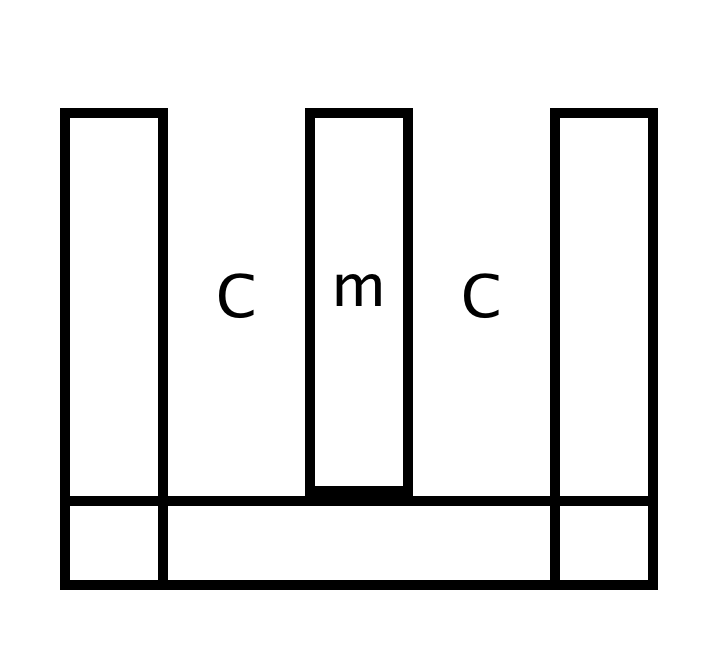
\includegraphics[keepaspectratio=true,scale=0.5]{accelerometer.png}  %skala och filnamn. 
  \end{center}
  \caption{Modell av accelerometer} %figurtext.
  \label{fig:accelerometer}
\end{figure}

En gyrosensor av MEMS-typ (Micro Electro-Mechanical System) utnyttjar att två lika stora massor som oscillerar konstant i motsatta riktningar påverkas av Corioliskraften vid rotation. Kraften verkar i olika riktningar på de två massorna vilket leder till en förändring i kapacitans.
Skillnaden i kapacitans har visat sig vara proportionell mot vinkelhastigheten, och därför går det att bestämma vinkelhastigheten med hjälp av ett gyro av denna typ \footnote{Introduction to MEMS gyroscopes. Solid State Technology, Insights for Electronics  Manufacturing (\url http://electroiq.com). \url{http://electroiq.com/blog/2010/11/introduction-to-mems-gyroscopes/}, hämtad 2014-05-06}. 

\subsubsection{Hjulsensorer}

Vid vissa tillfällen kan det vara så att avståndssensorer ej kan användas för att skatta rörelse relativt landmärken, exempelvis om alla landmärken är utanför sensorernas räckvidd. Man kan då behöva skatta sin rörelse med hjälp av någon annan sensor. En vanlig typ av sensor är då hjulsensorer. Hjulsensorer räknar hur många varv hjulen snurrat och skattar sedan avståndet roboten färdats utifrån detta. 

Ett problem med hjulsensorer är att de inte ger en helt korrekt hastighets- och distansskattning då hjulen ofta slirar mot underlaget.

\subsubsection{Andra typer av sensorer}

I denna rapport berör vi mest fallet att SLAM baseras på optiska avståndssensorer, hjulsensorer och gyro, men det finns även andra typer av sensorer som går att använda. Till exempel finns det implementeringar som använder sig av kameror för att finna landmärken och sedan använda dessa som referenser. Det krävs dock mer avancerade algoritmer för att finna lämpliga landmärken i detta fall \footnote{Karlsson, N.; Goncalves, L.; Munich, M.E.; Pirjanian, P.''The vSLAM Algorithm for Navigation in Natural Environments''. Evolution Robotics, Inc. Hämtad 28 mars 2014}.

Något som också provats är SLAM utan användning av någon typ av optisk utrustning och att istället förlita sig på känsel. Med hjälp av känselsensorer, som efterliknar djurs morrhår, försöka kartlägga ett helt mörklagt rum. Denna metod har dock inte gett så bra resultat med de tekniker som existerar i dag\footnote{Fox, C.; Evans, M.; Pearson, M.; Prescott, T. (2012)
''Tactile SLAM with a biomimetic whiskered robot''. 2012 IEEE International Conference on Robotics and Automation. Hämtad 28 mars 2014.
\url{http://ieeexplore.ieee.org/stamp/stamp.jsp?tp=&arnumber=6224813}
}. 

\subsubsection{Absolut positionsskattning}Tidigare nämndes exempel på metoder som använder sig av GPS. Detta i kombination med WiFi-signaler har använts till exempel i mobiltelefoner för att ge en positionsskattning med absolut referens för var enheten befinner sig. För att WiFi-SLAM ska fungera krävs att accesspunkten har information om positionsdata för sig själv, alternativt att den anslutna enheten har information om var aktuellt WiFi är tillgängligt.

I tillämpningar där positionen inte behöver skattas med så hög nogrannhet är GPS fullt tillräcklig och SLAM-algoritmer behöver därför inte implementeras. Om man däremot behöver mer nogrannhet och robusthet än vad GPS kan ge kan GPS användas som ett hjälpmedel för att snabbt uppskatta inom vilket område man befinner sig för att kraftigt förenkla SLAM-problemet. 


%------------------------------------------------
%--------------------Fördjupning-----------------
%------------------------------------------------
\newpage
\section{Skattningsmetoder för SLAM-problemet}
I denna fördjupande del går vi igenom metoder som kan användas för att utföra SLAM i en miljö lik den i problemställningen. Bland annat kommer tillståndsrepresentation och skattning av tillstånd med hjälp av observatörer samt kalmanfilter att tas upp.

%----------------------Tillståndsrepresentation av reglersystem------------------

\subsection{Tillståndsrepresentation av reglersystem}

Inom reglerteknik kan linjära system beskrivas på så kallad tillståndsform\footnote{Glad, Torkel och Ljung, Lennart (2006), \textit{Reglerteknik - Grundläggande teori}.}. I fallet med SLAM för en robot använder man robotens position och orientering som tillstånd, som beskrivits tidigare. Ett tidskontinuerligt linjärt ystem kan skrivas på tillståndsform enligt
\begin{gather}
\dot{x}=Ax+Bu \\
y=Cx+Du	
\label{equ:tillstand}
\end{gather}
där $A$, $B$, $C$ och $D$ är matriser.

Tillstånden för en robot mäts vid diskreta tidpunkter då datorer endast hanterar tidsdiskreta mätningar och ej kontinuerliga. I dessa fall är det bättre att använda sig av en tidsdiskret tillståndsbeskrivning
\begin{gather}
x_{n+1} = Ax_n + Bu_n \\
y_n = Cx_n + Du_n
\label{equ:disktillstand}
\end{gather}

Om systemet istället skulle vara icke-linjärt så går det inte att beskriva det på samma sätt utan man får använda sig av en olinjär tillståndsbeskrivning. 
\begin{gather}
	x_{t+1}=f(x_t,u_t)
	y_t=h(x_t,u_t)
\end{gather}

Man kan få en approximativ linjäriserad beskrivning av ett sådant system genom att använda sig av Taylorutveckling, vilket i slutändan leder till att $A$-, $B$-, $C$- och $D$-matriserna innehåller partiella derivator. Dessa matriser kallas jacobianer, $J$ och skrivs
\begin{gather}
	J= \begin{pmatrix}
	\frac{\partial f_1}{\partial x_1} & \dots & \frac{\partial f_1}{\partial x_n} \\
	  							\vdots &       & \vdots \\
	  \frac{\partial f_n}{\partial x_1} & \dots & \frac{\partial f_n}{\partial x_n}
	  \end{pmatrix}
	  \label{equ:jacobian}
\end{gather}

I ett praktiskt implementerbart system nyttjas till exempel sensorer som ger mätsignaler med en viss osäkerhet på mätdatan för att bestämma systemets tillstånd. Man kan därmed enbart skatta systemets tillstånd och inte exakt beräkna det. För att skatta tillståndet används ofta en så kallad observatör.

\subsubsection{Observatörer}

Inom reglerteknik används en observatör för att skatta tillståndsvariabler i ett givet system. Tillståndet för systemet (4)-(5) kan skattas med hjälp av observatören

\begin{gather}
\dot{\hat{x}} = Ax + Bu + K(y - C\hat{x})
\label{equ:observer}
\end{gather}

Skattningsfelet $\tilde{x}= x - \hat{x}$ ges då av differentialekvationen

\begin{gather}
\dot{\tilde{x}} = (A - KC)\tilde{x}
\label{equ:observerError}
\end{gather}

Genom att sedan välja olika $K$-matriser får observatören olika egenskaper i form av konvergenshastighet och störningskänslighet. 

\subsubsection{Tidskontinuerlig och tidsinvariant kalmanfilter}

Antag att systemet (4)-(5) påverkas av mätstörningen $e$ och systemstörningen $v$ som specificerades i problemformuleringen
\begin{gather}
\dot{x}=Ax+Bu+e \\
y=Cx+Du+v
\end{gather}

Skattningsfelet ges då istället av: 
\begin{gather}
\dot{\tilde{x}} = (A - KC)\tilde{x} + e - Kv
\end{gather}

Då $e$ och $v$ antas vara vita brus kan man, genom att utgå från störningarnas kovariansmatriser $R_1$ och $R_2$, beräkna skattningsfelets kovarians. Kovariansen hos skattnignsfelet minimeras sedan genom att välja 
\begin{gather}
K = PC^{T}R_{2}^{-1}
\end{gather}

där matrisen $P$ är den positivt semidefinita lösningen till 
\begin{gather}
AP + PA^{T} + R_{1} - PC^{T}R_{2}^{-1}CP = 0
\end{gather}

I många praktiska tillämpningar antas $R_{1}$ och $R_{2}$ vara diagonalmatriser för att förenkla implementeringar. Dessa matriser väljs sedan beroende på hur mycket systemet påverkas av yttre störningar av olika typ. 

\subsubsection{Tidsdiskret och tidsvariabelt kalmanfilter} Inom SLAM är både hastighet och störningskänslighet essentiellt och man använder därför en tidsvariabel $K$-matris. Det vanliga kalmanfiltret är tyvärr inte effektivt vid SLAM, eftersom filtret enbart kan användas för linjära system. För att skatta nästkommande tillstånd med variabel $K$-matris används därför vanligen ett utökat kalmanfilter vid implementeringar av SLAM. 

För att beskriva det utökade kalmanfiltret behöver vi först beskriva det tidsdiskreta och tidsvarianta kalmanfiltret. Systemet beskrivs då som 
\begin{gather}
x_{n+1} = Ax_n + Bu_n+e \\
y_n = Cx_n + Du_n + v
\end{gather}
och skattningen ges av
\begin{gather}
	\hat{x}_{n+1|n} = A_n\hat{x}_{n|n-1} + K_n(y_n-C_n) \\
	K_n=A_nP_{n|n-1}C_n^T([C_nP_{n|n-1}C_n^T+R_2)^{-1}	\\
	P_{n+1|n}=A_nP_{n|n-1}A_n^T+R_{1} 
	        -A_nP_{n|n-1}C_n^T(C_nP_{n|n-1}C_n^T+R_1)^{-1}C_nP_{n|n-1}A_n^T
\end{gather}
där $R_1$ och $R_2$ är kovariansmatriserna för $e$ respektive $v$. $A$-,$B$-,$C$- och $D$-matriserna varierar med tiden.  

\subsubsection{EKF - Det utökade kalmanfiltret}

Till skillnad från kalmanfiltret kan det utökade kalmanfiltret användas för att approximativt lösa icke-linjära SLAM-problem. Det som möjliggör detta är att filtrets matriser beräknas om för varje ny tillståndsskattning. Matriserna för filtret beräknas med hjälp av jacobianer (9), och systemet linjäriseras därmed kring varje skattat tillstånd för att kunna skatta nästa tillstånd. 

Initalt sätts kovariansen, $R$,till ett väldigt stort värde innan man vet vilken kovarians sina mätningar i miljön har. Därefter plockas mätdata in och man beräknar sin K-matris för att beräkna nästkommande tillstånd enligt: 

\begin{gather}
K[n+1] =  P[n]J[n]^{T}(J[n]P[n]J[n]^{T}+R[n])^{-1}
\end{gather}

Där J är jacobianen\label{equ:jacobian} som ges av partiella derivatorna hos mätdatat för avstånd till landmärken, $y[n] = h(x[n]^{r},m[n])$. \footnote{David Törnqvist. Estimation and Detection with Applications to Navigation.}

\newpage

\subsection{FastSLAM}
FastSLAM är en relativt modern teknik som använder ett så kallat partikelfilter för att filtrera mätdata, där varje tänkbart tillstånd för systemet ses som en partikel. De mest sannolika värdena sparas och de minst sannolika tillstånden förkastas. Man kallar det här för en omsampling då man utgår från en sampelmängd av tillstånd och sedan uppdaterar denna när man får nya mätningar. Antag att partikelfiltret plockar ut $N$ tillstånd ur den totala mängden tillstånd. 

\begin{gather}
x^i[n] \sim p(x[n]|y[1:n]),\;\;\;\;\;\; i = 1, ..., N
\end{gather}

 Totala sannolikheten för tillståndet kan alltså delas upp enligt: 

\begin{gather}
p(x[n],m) = p(x[n]|y[n])p(m|y[n])
\end{gather}

Där, som tidigare nämts, $x$ är robotens tillstånd, $m$ är landmärkens position och $y$ är mätningarna för givet tillstånd.  

Tillstånden körs sedan flera gånger genom filtret tills dess att man med tillräckligt stor sannolikhet kan bestämma kartans utseende. Metoden har visat sig effektiv i praktiken. Nackdelen med metoden är att man genom omsampling av mätvärdena förlorar mätinformation som skulle kunna vara korrekt. Beroende på hur filtret prioriterar är det möjligt att man får en skev bild av omgivningen. 

För att effektivisera filtreringen av mätvärden delas olika distinkt upptäckta objekt i robotens miljö in i olika zoner. Dessa zoner filtreras sedan individuellt för att få fram den mest sannolika positionen för objektet i zonen.

%------------------------------------------------
%------------Resultat och slutsatser-------------
%------------------------------------------------
\newpage
\section{Slutsats}

Till slut kan vi konstatera att SLAM används i många tillämpningar man kanske inte tänker på. Man kan också konstatera att algoritmerna, filtren och mjukvaran som används för att implementera SLAM ibland kan vara väldigt komplexa. Algoritmerna som viktar vilka partiklar ska sparas respektive förkastas kan byggas ut i stort sett hur mycket som helst. 

En sådan lösning skulle kunna baseras på en tillståndsrepresentation med ett tidsvariant, tidsdiskret Kalmanfilter. Genom att medelvärdesbilda sensordata kan man antagligen försumma mätstörningar och ändå få en acceptabel skattning av omgivningen utan partikelfilter. Reglerfel kan i sin tur sedan minimeras med bra modellering av hårdvaran implementeringen nyttjar. 

\section{Reflektion}

Sett från det perspektiv vi granskar SLAM-problemet, inom ett kandidatprojekt, är avancerade FastSLAM-algoritmer för att implementera. Det måste dock alltid finnas någon typ av filter i en SLAM-implementering. Då beräkningar man gjort tidigare under kartläggningen ger konflikt med nuvarande mätning om huruvida en vägg faktiskt finns där eller ej. Enklare fall av partikelfiltrering kommer alltså behöva lösas vid vår framtida implementering. Vi kommer då att lösa det genom att låta roboten besöka området på nytt och ta ett beslut utifrån de nya mätdata vi får in. 

Slutligen kan man säga att denna fördjupning inom SLAM givit oss bra förutsättningar att skapa en implementerbar metod för hur vår robot ska kartlägga sitt slutna område. Särskilt avsnitten om Kalmanfilter och tillståndsmodeller känns relevanta vid en enklare implementering. 

% --------------- Källförteckning ---------------------
\newpage 
\section*{Källförteckning} 
\addcontentsline{toc}{section}{Källförteckning}

Weinberg, Harvey (1999), ''Dual Axis, Low g, Fully Integrated Accelerometers'', \url{http://www.analog.com/library/analogdialogue/archives/33-01/accel/index.html}. Hämtad 2014-05-12.

David Törnqvist. Estimation and Detection with Applications to Navigation. PhD thesis, Linköping University, 2008, \url{http://urn.kb.se/resolve?urn=urn:nbn:se:liu:diva-14956}. Hämtad 15 april 2014.

FastSLAM: A Factored Solution to the Simultaneous
Localization and Mapping Problem, Stanford University. Hämtad 28 mars 2014.
\url{http://robots.stanford.edu/papers/montemerlo.fastslam-tr.pdf}

Fox, C.; Evans, M.; Pearson, M.; Prescott, T. (2012)
''Tactile SLAM with a biomimetic whiskered robot''. 2012 IEEE International Conference on Robotics and Automation. Hämtad 28 mars 2014.
\url{http://ieeexplore.ieee.org/stamp/stamp.jsp?tp=&arnumber=6224813}

Glad, Torkel och Ljung, Lennart. 2006. \textit{Reglerteknik - Grundläggande teori}. Upplaga 4:10. Lund. Studentlitteratur.

Gustavsson, Fredrik; Ljung, Lennart; Millnert, Mille. 2000. \textit{Signalbehandling}. Andra upplagan. Lund. Studentlitteratur.

Kandidatprojekt Y: Elektronikprojekt, Tävlingsregler för katläggningsrobot. Hämtad 28 mars 2014.  \url{https://drive.google.com/file/d/0B758zzcy4ZrTeG1wRTY4WG9lTDQ/edit?usp=sharing}

Karlsson, N.; Goncalves, L.; Munich, M.E.; Pirjanian, P.
''The vSLAM Algorithm for Navigation in Natural Environments''. Evolution Robotics, Inc. Hämtad 28 mars 2014:
\url{http://www.vision.caltech.edu/mariomu/research/papers/vSLAM-krs.pdf}

Risgaard, S; Blas, M.R (2005).
''SLAM for Dummies, A Tutorial Approach to Simultaneous Localization and Mapping''. 
Hämtad 28 mars 2014:
\url{http://ocw.mit.edu/courses/aeronautics-and-astronautics/16-412j-cognitive-robotics-spring-2005/projects/1aslam_blas_repo.pdf}

Smith, R.C.; Cheeseman, P. (1986). ''On the Representation and Estimation of Spatial Uncertainty''. The
International Journal of Robotics Research, 5(4), sida 56–68. Hämtad
28 mars 2014:
\url{http://www.frc.ri.cmu.edu/~hpm/project.archive/reference.file/Smith&Cheeseman.pdf}

\subsection{Websidor}

Piezoelectricity, Wikipedia. \url{http://en.wikipedia.org/wiki/Piezoelectricity}. Hämtad 2014-05-12.

Openslam.org
\url{http://www.openslam.org/}

Introduction to MEMS gyroscopes. Solid State Technology, Insights for Electronics  Manufacturing (\url http://electroiq.com). \url{http://electroiq.com/blog/2010/11/introduction-to-mems-gyroscopes/}, hämtad 2014-05-06

\end{document}